\documentclass[11pt,letterpaper]{article}

\input{../../../../.config/latex/preamble_v1.tex}
\lightmode

\begin{document}

\section*{CS 124 Homework 5: Spring 2022}

\textbf{Your name:} Lev Kruglyak

\textbf{Collaborators:} Adam Mohamed, Sahil Kuchlous

\textbf{No. of late days used on previous psets: 10}\\
\textbf{No. of late days used after including this pset: 12}

Homework is due Wednesday at midnight ET. You are allowed up to {\bf twelve} (college)/{\bf forty} (extension school) late days through the semester, but the number of late days you take on each assignme\
nt must be a nonnegative integer at most {\bf two} (college)/{\bf four} (extension school).

Try to make your answers as clear and concise as possible;
style may count in your grades. Assignments must be submitted in pdf format on Gradescope. If you do assignments by hand, you will need to scan in your results to turn them in.

You can collaborate with other students that are currently enrolled in this
course in brainstorming and thinking through approaches to solutions but you should write
the solutions on your own: you must wait one hour after any collaboration or use of notes
from collaboration before any writing in your own solutions that you will submit. 

For all homework problems where you are asked to give an algorithm, you must prove the correctness
of your algorithm and establish the best upper bound that you can give for the running time. Generally
better running times will get better credit; generally exponential time algorithms (unless specifically asked
for) will receive no or little credit. You should always write a clear informal description of your algorithm
in English. You may also write pseudocode if you feel your informal explanation requires more precision
and detail, but keep in mind pseudocode does NOT substitute for an explanation. Answers that consist
solely of pseudocode will receive little or not credit. Again, try to make your answers clear and concise.

\pagebreak
\begin{problem}
    PhyllisNotes Incorporated sells PhyllisNotes$^{\mathrm{TM}}$ subscriptions to CS124 students at \$78.50 per semester. Andrew, the CTO, runs the online platform where subscribed users can view PhyllisNotes$^{\mathrm{TM}}$. Each student can log in to their PhyllisNotes$^{\mathrm{TM}}$ account using only a password (Andrew has not discovered the concept of usernames). To combat intellectual property theft, Andrew has implemented a strict policy where each student can only log in from their own laptop. This policy is enforced via the use of a hash table, which hashes students' passwords and stores the IP address of the laptop logging in with that password. Students who log in to their PhyllisNotes$^{\mathrm{TM}}$ accounts from someone else's laptop will immediately have their accounts closed for violating the terms of service. Each entry of Andrew's hash table stores (at most) one IP address, so in case of hash collisions, however, Andrew's design contains a major flaw (not surprising for someone with no college degree). If Student A creates and logs into an account using a password that hashes to the same value as the password of Student B, the website will mistake Student A for Student B, believe that Student B logged in from Student A's laptop, and close Student B's account. Assume that each student enters their own account using only their own laptop, and every student whose account has been wrongfully closed will file a lawsuit against PhyllisNotes Incorporated.
    \begin{enumerate}[(a)]
        \item {\bf (10 points)} There are 237 students in CS124, 100 of which have indicated in a survey that they will subscribe to PhyllisNotes$^{\mathrm{TM}}$. How large must Andrew's hash table be so that the probability that PhyllisNotes Incorporated gets sued is at most 1\%? (You'll likely want to use a calculator or program.)
        \item {\bf (10 points)} Unfortunately, as nearly all of the company's data storage capacity is being used to store and back up PDFs of PhyllisNotes$^{\mathrm{TM}}$, Andrew is unable to build a large enough hash table as required in part (a). Instead, he will need to estimate the number of lawsuits that will be filed.
        Suppose there are $m$ students this year who will subscribe to PhyllisNotes$^{\mathrm{TM}}$, and the
        hash table has $n$ slots. Calculate the expected number of lawsuits that will be filed this
        year, as a function of $m$ and $n$.
    \end{enumerate}
\end{problem}

\begin{solution}
    \textbf{(a)} Suppose we have a hash table of size $N$. The number of students in this case is $n=100$, and say we would like the propability of getting sued to be less than $\epsilon = 0.01$. Recall from lecture that the probability of a hash collision is
    \[
        P(n, N) = 1-\prod^{n-1}_{k=0}\left(1-\frac{k}{N}\right)
    .\] 
    Using the first order approximation $e^x\approx 1+x$, we get the approximation 
    \[
        P(n,N)\approx 1-\prod^{n-1}_{k=0}\left(e^{-k /N}\right) = 1-e^{-\frac{1}{N}\left(\sum^{n-1}_{k=0}k\right)} = 1-e^{-n(n-1) /2N} \approx 1-e^{-\frac{n^2}{2N}}
    .\] 
    Thus if we want $P(n,N)\leq \epsilon$, we can solve $1-e^{-\frac{n^2}{2N}}=\epsilon$ for $N$ which gives $N=-\frac{n^2}{2\log(1-\epsilon)}$. So for our values, we get $N\approx 497,495$. Refining this further using a calculator, we get an exact value for the $\epsilon$ cutoff point, which is $N=492,555$. Notice that $P(n,492,555)\approx 0.00999998$ whereas $P(n,492,554)\approx 0.01$. So the hash table should have at least $492,555$ entries, or a bit less than $19$ bits per hash.

    \textbf{(b)} The probability of a slot being empty is $\left(1-\frac{1}{n}\right)^m$, so the expected number of empty slots is $n\left(1-\frac{1}{n}\right)^m$. So the expected number of slots with at least one entry is $n-n\left(1-\frac{1}{n}\right)^m$. Thus the expected number of lawsuits is
    \[
        m - n + n\left(1-\frac{1}{n}\right)^m
    .\]  
\end{solution}

\pagebreak
\begin{problem}
    Suppose each person gets an independent uniformly random hash value from the range $[1\ldots n]$.  (For the case of birthdays, $n$ would be 365.) 
    \begin{enumerate}[(a)]
        \item {\bf (10 points)} Show that for some constant $c_1$, when there are at least $c_1 \sqrt{n}$ people in a room, the probability that no two have the same hash value is at most $1/2$. (Note that the hints below may be relevant for any part of the problem.)
        \item {\bf (10 points)} Similarly, show that for some constant $c_2$ (and sufficiently large $n$), when there are at most $c_2 \sqrt{n}$ people in the room, the probability that no two have the same hash value is at least 1/2. 
\end{enumerate}
\end{problem}

\begin{solution}
    \textbf{(a)} Recall from lecture that the probability of there being no hash collisions among $m$ elements with $n$ total hash values is
    \[
        P(m,n)=\prod^{m-1}_{k=0}\left(1-\frac{k}{n}\right)
    .\] 
    Using the upper bound $e^x \geq 1+x$, we have
    \[
        \prod^{m-1}_{k=0}\left(1-\frac{k}{n}\right) \leq \prod^{m-1}_{k=0}e^{-\frac{k}{n}}=e^{\left(-\frac{1}{n}\sum^{m-1}_{k=0}k\right)}=e^{-\frac{m(m-1)}{2n}}\leq e^{-\frac{(m-1)^2}{2n}}
    .\]
    Note that this is a monotonically decreasing function, so to find an $m$ for which $P(m',n)\leq 1/2$ whenever $m'\geq m$, it suffices to pick any $m$ with $P(m,n)\leq 1/2$. Using the upper bound, we have
    \[
        e^{-\frac{(m-1)^2}{2n}}=\frac{1}{2}\implies m=1+\left(\sqrt{2\log 2}\right)\sqrt{n} 
    .\] 
    To put this into the $c_1\sqrt{n}$ form, note that for example $\left(\sqrt{3\log 2}\right)\sqrt{n}\geq 1+\left(\sqrt{2\log 2}\right)\sqrt{n}$ works. So the constant $c_1=\sqrt{3\log 2}$ works.
    
    \textbf{(b)} Using the lower bound $e^{-x-x^2}\leq 1-x$, for $x\leq 1/2$ we get the lower bound
    \[
        \begin{aligned}
            \prod^{m-1}_{k=0}\left(1-\frac{k}{n}\right)\geq \prod^{m-1}_{k=0}e^{-\frac{k}{n}-\frac{k^2}{n^2}} = e^{-\frac{1}{n}\sum^{m-1}_{k=0}k}e^{-\frac{1}{n^2}\sum^{m-1}_{k=0}k^2}&=e^{-\frac{m(m-1)}{2n}}e^{-\frac{m(m-1)(2m-1)}{6n^2}}\\&\geq e^{-\frac{m^2}{2n}}e^{-\frac{m^3}{3n^2}}
            \geq e^{-\frac{m^2}{n}}.
        \end{aligned}
    \] 
    Notice that we don't really care about the cases when $k/n > 1 /2$ because we can make our lower bound so that $m\leq n/2$. Now solving for a lower bound we get
    \[
        e^{-\frac{m^2}{n}} = \frac{1}{2} \implies m = \left(\sqrt{\log 2}\right)\sqrt{n}
    .\] 
    So $c_2=\sqrt{\log 2}$ works. Notice that $\frac{\left(\sqrt{\log 2}\right)\sqrt{n}}{n}\leq \frac{1}{2}$ so the approximation works here. 
\end{solution}

\pagebreak
\begin{problem}\noindent
    \begin{enumerate}[(a)]
        \item {\bf (5 points)} In our description of Bloom filters in class, we could only add and look up items. Suppose we try to implement deletion of an item from a Bloom filter by changing the corresponding elements to 0s. Give an example sequence of operations (adds, deletes, and lookups) for which this Bloom filter has both a false positive and a false negative.
        \item {\bf (15 points)} Counting Bloom filters are a variant of Bloom filters where you do not use an array of bits, but an array of small counters. Instead of changing 0s to 1s when an element hashes to a Bloom filter location, you increment the counter. To delete an element, you decrement the counter.  To check if an element is in the set, you just check if all of the counter entries are bigger than 0; if they are, then you return the element is in the set. If you see a 0, you say that the element is not in the set. Deletions will work properly for a Counting Bloom filter as long as the counters never overflow;  once a counter overflows, you would not have an accurate count of the number of elements currently hashed to that location. A standard choice in this setting in practice to use 4 bit counters. Find an expression for the probability that a specific counter overflows when using 4 bit counters when $n$ elements are hashed into $m$ total locations using $k$ hash functions.  (You may have a summation in your expression.) Calculate this probability when $m/n = 8$ and $k=5$, for $n=1,000, 10,000,$ and $100,000$, and calculate the expected number of counters that overflow for each case.  
        \item {\bf (5 points)} Suppose that you use $m$ counters for $n$ elements and $k$ hash functions for a Counting Bloom filter.  What is the false positive probability (assuming there has never been an overflow), and how does it compare with the standard Bloom filter? 
    \end{enumerate}
\end{problem}

\begin{solution}
    \textbf{(a)} Suppose we try to encode a set of $2$ digit numbers into a $10$-bit Bloom filter. We'll use a simple hash function, the first one sends a two digit number to its first digit, the second hash functions sends a two digit number to its second digit. So for example $12$ would set the 2nd and 3rd bits of the filter. If we wanted to encode $12$, $23$, $45$, and $56$, the Bloom filter would be $0111111000$. Now suppose we removed $23$. Then the Bloom filter would be $0100111000$. We claim that this filter has both false positives and negatives. An example of a false positive is $46$ since both the $4$ and $6$ bits are set. A false negative is $12$, since the $2$ bit isn't set. (It was unset by removing $23$)
    
    \textbf{(b)} The total number of increments made by a hash function is $nk$. Since the number of slots is $m$, the probability that a given slot is incremented exactly $q$ times is
    \[
        \binom{nk}{q}\left(\frac{1}{m}\right)^q\left(\frac{m-1}{m}\right)^{nk-q} = \binom{nk}{q}\frac{(m-1)^{nk-q}}{m^{nk}}
    .\] 
    Thus, the probability that a slot at least $16$ increments (i.e. overflows) is
    \[
        1-\sum^{15}_{q=0}\binom{nk}{q}\frac{(m-1)^{nk-q}}{m^{nk}}
    .\] 
    We can calculate the desired values, putting them in a table:
    \begin{table}[htpb]
        \centering
        \begin{tabular}{|c|c|c|}
        \hline
        $n$ & probability of overflow & expected overflows\\
        \hline
        1,000 & 0.272065 & 272\\
        \hline
        10,000 & 0.272059& 2721\\
        \hline
        100,000 & 0.27058& 27206\\
        \hline
        \end{tabular}
    \end{table}
    
    \textbf{(c)} The false positivity rate will be the same assuming no overflows and deletions, since the lookup method for both filters simply checks if the counter/bit is nonzer
\end{solution}

\pagebreak
\begin{problem}
    For the document similarity scheme described in class, it would be better to store fewer bytes per document.  Here is one way to do this, that uses just 48 bytes per document: take an original sketch of a document, using 84 different permutations.  Divide the 84 permutations into 6 groups of 14.  Re-hash each group of 14 values to get 6 new 64 bit values.  Call this the {\em super-sketch}.  Note that for each of the 6 values in the super-sketch, two documents will agree on a value when they agree on all 14 of the corresponding values in the sketch. 
    \begin{enumerate}[(a)]
        \item {\bf (5 points)} Why does it make sense to simply assume that this is the only time a match will occur?
        \item {\bf (15 points)} Consider the probability that two documents with resemblance $r$ agree on two or more of the six sketches.  Write equations that give this probability and graph the probability as a function of $r$. Explain and discuss your results.
        \item {\bf (10 points)} What happens if instead of using a 64 bit hash value for each group in the supersketch, we only use a 16 bit hash?  An 8 bit hash?
    \end{enumerate}
\end{problem}

\begin{solution}
    \textbf{(a)} We hash the super sketches into a $64$-bit hash to check if they match, so the probability that there would be a collision is neglibly small.

    \textbf{(b)} First, note that the probability that some pair of sketches agree is equal to the probablity that all $14$ values are the same, which is $r^{14}$. Thus the probaility that none of the sketches agree is $(1-r^{14})^6$. Similarly, the probability that exactly one of the sketches agree is $6r^{14}(1-r^{14})^5$. Thus, the probability that two or more of the sketches agree is
    \[
        P(r)=1-(1-r^{14})^6 - 6r^{14}(1-r^{14})^5
    .\]  
    Graphing this probability as a function of the resemblance, we get
    \begin{center}
        \begin{tikzpicture}
            \begin{axis}[
                axis lines = left,
                xlabel = \(r\),
                ylabel = {\(P(r)\)},
            ]
            \addplot[color=red, domain=0:1, samples=200, very thick]{1-(1-x^14)^6 - 6*x^14*(1-x^14)^5};
            \end{axis}
            \end{tikzpicture}
    \end{center}
    This graph validates the algorithm as a good algorithm for measuring resemblance because there is a very sharp rise in probability of a match as the resemblance gets high. So if two documents have a resemblance higher than $0.9$, there is a high chance that they would be detected by the algorithm.

    \textbf{(c)} Decreasing the hash size enough means that we must drop the assumption that two documents only will agree on a value if they agree on all $14$ values. So letting $B$ be the number of bits in the hash, the probability that a pair of sketches agree is now
    \[
        r^{14}+\frac{1-r^{14}}{2^B}.
    \] 
    This is because there is a $1/2^B$ chance of a false negative. We can substitute this expression into $P(r)$ to get
    \[
        P(r,B)=1-\left(1-\left(r^{14}+\frac{1-r^{14}}{2^B}\right)\right)^6-6\left(r^{14}+\frac{1-r^{14}}{2^B}\right)\left(1-\left(r^{14}+\frac{1-r^{14}}{2^B}\right)\right)^5
    .\]  
    Graphing this for several values of $B$, we get
    \begin{center}
        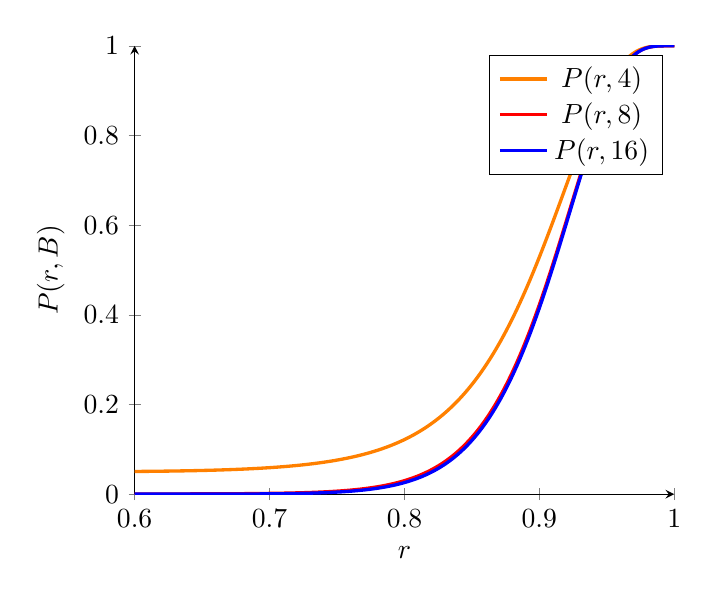
\begin{tikzpicture}
            \begin{axis}[
                axis lines = left,
                xlabel = \(r\),
                ylabel = {\(P(r, B)\)},
            ]
            \addplot[color=orange, domain=0.6:1, samples=200, very thick]{1-(1-(x^14+(1-x^14)/(2^4)))^6 - 6*(x^14+(1-x^14)/(2^4))*(1-(x^14+(1-x^14)/(2^4)))^5};
            \addlegendentry{\(P(r,4)\)}
            \addplot[color=red, domain=0.6:1, samples=200, very thick]{1-(1-(x^14+(1-x^14)/(2^8)))^6 - 6*(x^14+(1-x^14)/(2^8))*(1-(x^14+(1-x^14)/(2^8)))^5};
            \addlegendentry{\(P(r,8)\)}
            \addplot[color=blue, domain=0.6:1, samples=200, very thick]{1-(1-(x^14+(1-x^14)/(2^16)))^6 - 6*(x^14+(1-x^14)/(2^16))*(1-(x^14+(1-x^14)/(2^16)))^5};
            \addlegendentry{\(P(r,16)\)}
            \end{axis}
            \end{tikzpicture}
    \end{center}
    Notice that only lowering the hash size to something like $4$ bits significantly affects the efficacy of the algorithm, for hashes larger than $8$ bits the graph is basically the same as the $64$ bit hash. So for practical purposes, an $8$ bit hash suffices.
\end{solution}

\pagebreak
\begin{problem}
    Recall the fingerprinting algorithm presented in lecture 15 for determining whether a pattern of length $k$ appears in a document of length $n$ characters, each a number between 0 and 9: we hash the pattern by taking the decimal number it represents mod $p$; we hash each substring of length $k$ of the document by taking the decimal number it represents mod $p$, and, for every hash match, we compare the corresponding place in the document to the pattern, character by character, stopping if we find an instance of the pattern. For instance, comparing [3,1,4,1,5] to [3,1,4,1,5] takes 5 comparisons of characters (and then we can stop the algorithm, having found an occurrence of the pattern), and comparing [3,1,4,1,5] to [3,1,4,2,8] takes 4 comparisons of characters ([3,1,4,x]) (but we must move on to checking any other hash matches, in case one of them is a match).
 
    Instead of choosing a random prime number for $p$, say that we use some fixed prime number $p$ that is made public. Sara knows $p$ and wants to slow down your algorithm, so she is trying to construct a document and pattern that force you to do many comparisons of characters.
    \begin{enumerate}
        \item {\bf (5 points)} Suppose $p = 1249$, the pattern $P$ is $[3,1,4,1,5,9,2,6]$ (so $k=8$), and the document $D$ is $[1,4,6,8,3,4,8,3,1,8,6,4,3,1,5,9,7,0,3,1,4,1,7,1,7,5,1,1,3,2]$ (so $n=30$). The algorithm makes 11 comparisons of characters. What are those comparisons? 
        \item {\bf (12 points)} Give an asymptotic upper bound on the number of comparisons of characters that the algorithm performs in terms of the length $n$ of the document, the length $k$ of the pattern, and the prime $p$. 
        \item {\bf (12 points)} Give a family of examples (each consisting of a document, a pattern, and $p$) that require asymptotically as many comparisons of characters as possible. 
    \end{enumerate}

    For full credit, your bound should be tight: that is, your answers to the above questions should asymptotically match and be correct. Correctly-proven bounds that don't quite match are eligible for partial credit.
\end{problem}

\begin{solution}
    \textbf{(a)} Calculating the rolling hash function $H_{1249}(x)=x\mod 1249$, we get
    \begin{center}
        \begin{tabular}{|c|c|c|c|}
        \hline
        $x$ &$H_{1249}(x)$ & $x$& $H_{1249}(x)$\\
        \hline
        31415926 & \textcolor{red}{1078} & &\\
        \hline
        \hline
        14683483 & 239& 64315970 & 1213\\
        46834831 & \textcolor{red}{1078} &  43159703 & 508\\
        68348318 & 540 & 31597031 & \textcolor{red}{1078}\\
        83483186 & 26 & 15970314 & 600\\
        34831864 & 1001 &  59703141 & 941\\
        48318643 & \textcolor{red}{1078} & 97031417 & 354\\ 
        83186431 & 533 & 70314171 & 467\\
        31864315 & 1076 & 31417175 & \textcolor{red}{1078}\\ 
        18643159 & 585 & 14171751 & 597\\ 
        86431597 & 797 & 41717511 & 911\\
        71751132 & \textcolor{red}{1078} & & \\ 
        \hline
        \end{tabular}
    \end{center} 
    Since we compare $31415926$ to $46834831$, $48318643$, $71751132$, $31597031$, and $31417175$, we only have to do $11$ comparisons.   
    
    \textbf{(b)} Note that the number of $k$-length substrings is $n-k$, and each of these require at most $k$ comparisons, so an upper bound for the number of comparisons is $O(k(n-k))$. This bound can be made tighter, but doing this requires solving complicated modular equations with many variables.
    
    \textbf{(c)} Consider the patterm $P=[0,\ldots,0,p]$ and document $D=[0,\ldots,0]$ with prime $p$. Then clearly the hash of $P$ is zero modulo $p$, and the hash of any substring is also zero, so we check with all possible substrings. Lettting $k$ be the length of $P$ and $n$ be the length of $D$, it should be clear that we need to make $(n-k)(k-1)$ comparisons which asymptotically converges to $k(n-k)$. 
\end{solution}

\end{document}